\documentclass[11pt,a4paper,normalphoto,withhyper]{altareport}


%%%%%%%%%% PACKAGES %%%%%%%%%%
\usepackage[utf8]{inputenc}
\usepackage{setspace} %1.5 line spacing
\usepackage{notoccite} %% Citation numbering
\usepackage{lscape} %% Landscape table
\usepackage{caption} %% Adds a newline in the table caption
\usepackage{amssymb}
\usepackage{mathtools}
\usepackage[numbered,framed]{matlab-prettifier} % To add code listings from matlab
\usepackage[export]{adjustbox}
\usepackage{biblatex}

\addbibresource{references.bib} % Bibliography 


%% The paracol package lets you typeset columns of text in parallel
\usepackage{paracol}
\usepackage[none]{hyphenat}

%% Document and Theme Fonts
\usepackage[rm]{roboto}
\usepackage[defaultsans]{lato}
%\usepackage{sourcesanspro}



%%%%%%%%% Karnaugh Map Package & Settings %%%%%%%%%
\usetikzlibrary{matrix,calc}
\usepackage{karnaugh-map}

\colorlet{LightRed}{red!60!}
\colorlet{LightBlue}{blue!60!}
\colorlet{LightYellow}{yellow!60!}
\colorlet{LightGreen}{green!60!}
\colorlet{LightOrange}{orange!60!}


%%%%%%%%%% USEFUL SETTINGS %%%%%%%%%%
%% Change some font sizes, this will override the defaults
% \renewcommand{\familydefault}{cmr}  % choose your font here
\renewcommand{\ReportTitleFont}{\Huge\bfseries} %% Title Page - Main Title
\renewcommand{\ReportSubTitleFont}{\huge\bfseries} %% Title Page - Sub-Title
\renewcommand{\ReportSectionFont}{\LARGE\bfseries} %% Section Title
\renewcommand{\ReportSubSectionFont}{\large\bfseries} %% SubSection Title
\renewcommand{\ReportEmphasisFont}{\bfseries}
\renewcommand{\FootNoteFont}{\footnotesize} %% Footnotes and Header/Footer

%% Change the bullets for itemize and rating marker
\renewcommand{\itemmarker}{{\small\textbullet}}
\renewcommand{\ratingmarker}{\faCircle}

%% Change the page layout
\geometry{left=1.5cm,right=1.5cm,top=3cm,bottom=3cm,columnsep=8mm}

\onehalfspace   % 1.5 line spacing

%% Depending on your tastes, you may want to make fonts of itemize environments slightly smaller
% \AtBeginEnvironment{itemize}{\small}

\definecolor{CommentGreen}{HTML}{228B22}

%% This makes " an escape character to write in matlab editor font
\lstMakeShortInline[style=Matlab-editor]" 

%%%%%%%%% Arduino Language Settings %%%%%%%%%
\lstset{%
  language = Octave,
  backgroundcolor=\color{white},   
  basicstyle=\color{body}\footnotesize\ttfamily,       
  %breakatwhitespace=false,         
  breaklines=true,                                
  commentstyle=\color{CommentGreen},
  columns=fullflexible,
  escapeinside={\%*}{*)},
  extendedchars=true,
  frame=leftline,
  keepspaces=true,
  keywordstyle=\color{LightBlue},
  numbersep=5pt,
  numberstyle=\footnotesize\color{gray},
  rulecolor=\color{black},
  rulesepcolor=\color{black},
  showtabs=true,
  stringstyle=\color{LightBlue},
  tabsize=2,                       
  title=\lstname,
  emphstyle=\bfseries\color{LightOrange}%  style for emph={} 
} 

%%%%% language/example specific settings: %%%%%
\lstdefinestyle{Arduino}{%
    language = C++,
    keywords={void, int, boolean, char, unsigned, long, uint32_t, volatile, byte, uint8_t, HIGH, OUTPUT, LOW, INPUT},%                 define keywords
    morecomment=[l]{//},%             treat // as comments
    morecomment=[s]{/*}{*/},%         define /* ... */ comments
    emph={WiFi, Serial, IPAddress, Adafruit_NeoPixel, setFrequency, println, print, delay, digitalWrite, pinMode, available, digitalPinToInterrupt, attachInterrupt, detachInterrupt, analogRead, NEO_GRB, NEO_KHZ800, noInterrupts, interrupts, strstr, endPacket, beginPacket, remoteIP, remotePort, APClientMacAddress, Color}%        keywords to emphasize
}


%%%%%%%%%%%%%%%%%%%%%%%%%%%%%%%%%%%%%%%%%%%
%%%%%%%%%% THEMES %%%%%%%%%%#

%% Standard theme options are below, leave blank for B&W / no colours (BoringDefault). Note the theme will be set to default if you enter a non-exsistant theme name.
\SetTheme{UUTheme}
%% ChillBlue
%% GreenAndGold
%% WisePurple
%% PastelRed
%% UUTheme
%% BoringDefault (Leave blank / enter anything not found above)


%%%%%%%%%% TITLE PAGE INFO %%%%%%%%%%
\ReportTitle{Academic Report Template}
\SubTitle{Assignment One}
\Author{Joe Bloggs - B00111111}
\ReportDate{\today}
\ModCoord{Dr. John McLecturer}

\begin{document}

\MakeReportTitlePage

%%%%% CONTENTS %%%%%
\pagenumbering{roman} % Start roman numbering
\setcounter{page}{1}

%%%%%%%%%% YOUR NAME, PROFESSION, PORTRAIT, CONTACT INFO, SOCIAL MEDIA ETC. %%%%%%%%%%
\name{Andrew Simon Wilson}
\tagline{Undergraduate BEng Mechatronic Engineer, Ulster University}

\personalinfo{
  \email{andrew.s.wilson@tutanota.com}
  \linkedin{andrew-simon-wilson} 
  \github{AS-Wilson}
  \phone{+44 7930 403 218}
}

%% You can add multiple photos on the left or right
% \photoR{3cm}{Images/a-wilson-potrait.jpg}
% \photoL{3cm}{Yacht_High,Suitcase_High}


\section*{Author Details}
\makeauthordetails

\section*{Co-Author Details}
\name{Michael Jennings MEng MEng}
\tagline{PhD Candidate, Ulster University}

\personalinfo{
  \email{mjennings061@gmail.com}
  \linkedin{mjennings061} 
  \github{mjennings061}
  \phone{+44 7930 403 219}
}
\makeauthordetails
%% Table of contents print level -1: part, 0: chapter, 1: section, 2:sub-section, 3:sub-sub-section, etc.
\setcounter{tocdepth}{2} 
\tableofcontents %% Prints a list of all sections based on the above command
%\listoffigures %% Prints a list of all figures in the report
%\listoftables %% Prints a list of all tables in the report




%%%%%%%%%% DOCUMENT CONTENT BEGINS HERE %%%%%%%%%%

%%%%% INTRO %%%%%
\section*{Introduction}
Here is and example how you cite throughout the document\cite{JenningsWilson2021}, the default bibliography format is IEEE Transactions.
\newpage
\pagenumbering{arabic} % Start document numbering - roman numbering




%%%%% COURSEWORK THREE %%%%%
\section{Simple Figure Example}
Here is an example of a figure, and how to insert one into your document see below in Figure \ref{fig:Example_Figure_Circuit}:
\begin{figure}[h]
	\centering
	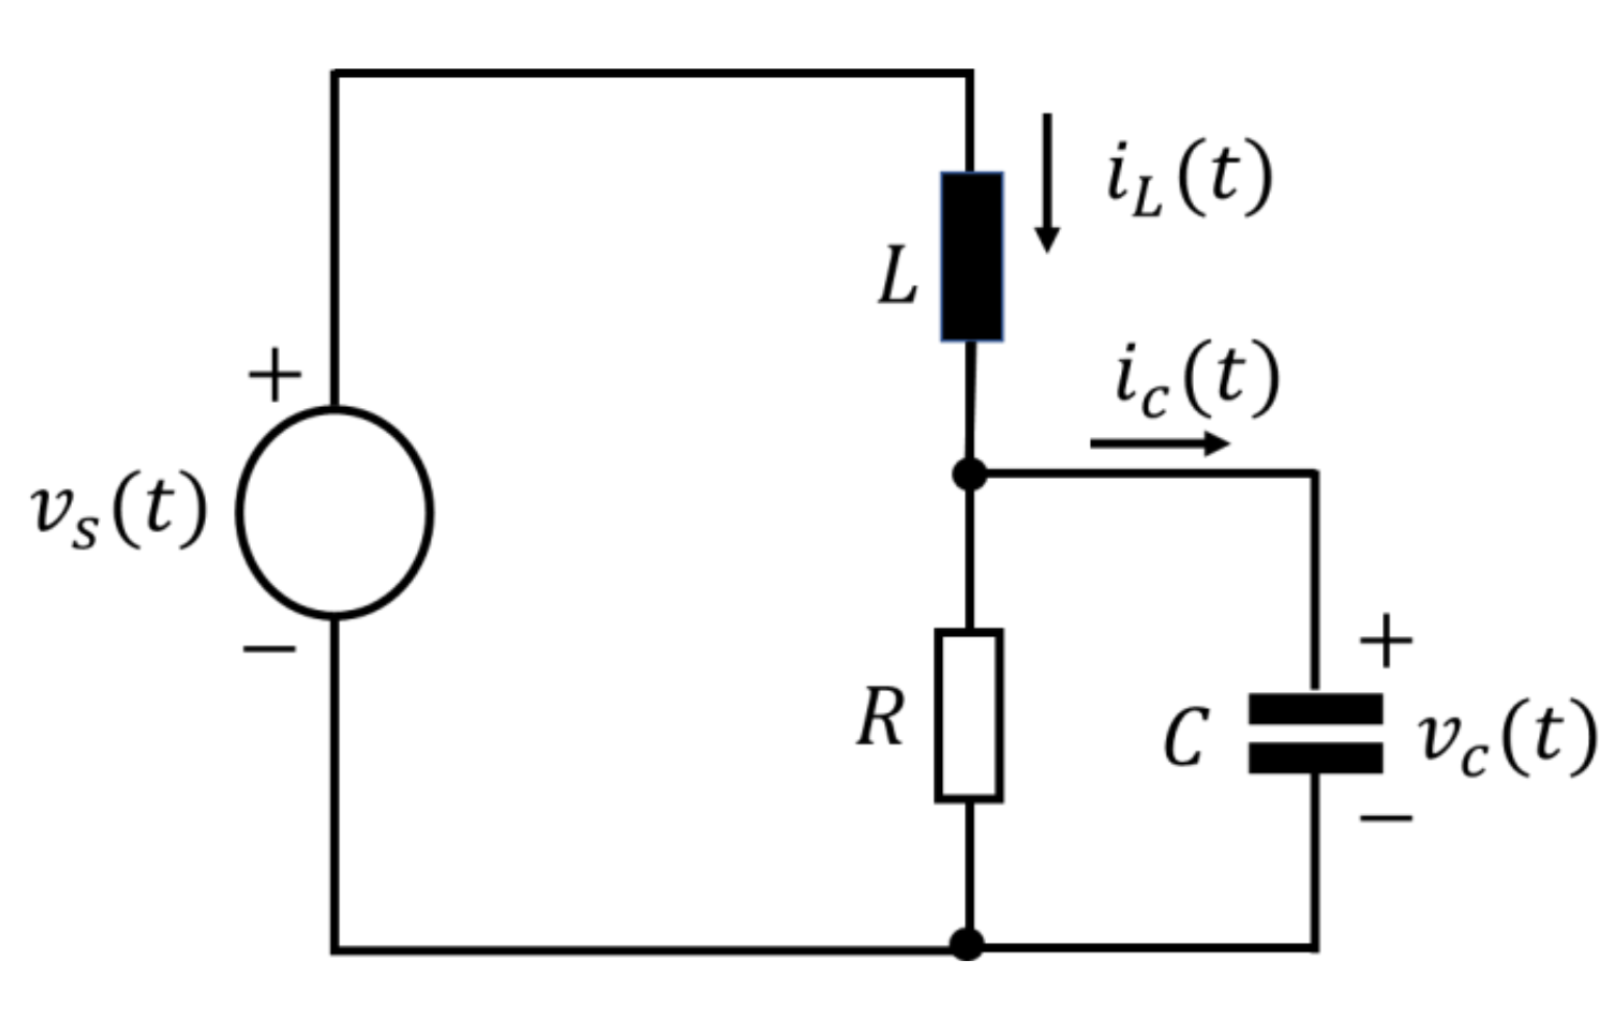
\includegraphics[width=6cm]{Images/CW3_Circuit_One.png}
	\caption{Circuit One, for reference.}  %% Caption for your figure
	\label{fig:Example_Figure_Circuit}
\end{figure}




\section{Equations}
\subsection{Simple Equations}
Perhaps you need to enter some equations in your work, as shown in Equations \ref{eqn:example_1} and \ref{eqn:example_2}

\begin{gather} %% Use this environment to center all the equations
	\frac{dI_L(t)}{dt}=-\frac{1}{L}V_C(t)+\frac{1}{L}V_S(t)
	\label{eqn:example_1}\\
	\frac{dV_C(t)}{dt}=\frac{1}{C}I_L(t)-\frac{1}{RC}V_C(t)
	\label{eqn:example_2}\nonumber\\
\end{gather}


\subsection{Matrices and Math Intertext}
Or perhaps you want some matrices (Equation \ref{eqn:example_matrice}),  some text between your equations whilst you show your working out, as seen culminating in Equation \ref{eqn:example_intertext}.

\begin{equation} %% Use this environment for most equations
		\begin{bmatrix}
			\dot{I}_L(t)\\
			\dot{V}_C(t)
		\end{bmatrix}
		=
		\begin{bmatrix}
			0&-\frac{1}{L}\\
			\frac{1}{C}&-\frac{1}{RC}
		\end{bmatrix} 
		\begin{bmatrix}
			I_L(t)\\
			V_C(t)
		\end{bmatrix}
		+
		\begin{bmatrix}
			\frac{1}{L}\\
			0
		\end{bmatrix}V_S(t)
		\label{eqn:example_matrice}
\end{equation}

\begin{align} %% Use this environment along with &'s to place align all the equations
	\intertext{Performing a Laplace transform on the general formulas will produce:}
	\mathcal{L} \{ \dot{X}=AX+BU \} &= sX(s)=AX(s)+BU(s)\nonumber\\\
	\mathcal{L} \{ Y=CX+DU \}  &= sY(s)=CX(s)+DU(s)\nonumber
	\intertext{The state equation can be rearranged to give:}
	X(s)&[Is-A]=BU(s)\nonumber\\\
	X(s)&=[Is-A]^{-1}BU(s)\nonumber\
	\intertext{Substituting this into the output equation gives a general solution:}
	Y(s)&=C[Is-A]^{-1}BU(s)+DU(s)\nonumber\\\
	\frac{Y(s)}{U(s)}&=C[Is-A]^{-1}B+D
	\label{eqn:example_intertext}
\end{align}


\subsection{Karnaugh Maps}
Below in Table \ref{tab:example_Karnaugh_Map} is a very complex example of how to do Karnaugh maps I used for an assignment, be very careful when reading the code for this entry as the tikz karnaugh map library accepts the inputs for the cells in a very strange order. There is plenty there to give you some examples to put this in your own report.
\bigskip

\begin{table}[h!]
	\begin{center}
    \caption{Karnaugh Map}
    \label{tab:example_Karnaugh_Map}
    \begin{tabular}{p{4cm} p{3.8cm} | p{4cm} p{3.8cm}}
    
      \multicolumn{2}{c}{Output $A$} & \multicolumn{2}{c}{{Output $B$}} \\
      %% A %%
      \parbox[c]{5mm}{\resizebox{4cm}{!}{
      \begin{karnaugh-map}[4][4][1][$x_3x_4$][$x_1x_2$]
      	\manualterms{1,0,1,1, 0,1,1,1, 1,1,x,x, x,x,x,x}
      	\implicant{3}{6}
      	\implicant{5}{7}
      	\implicant{8}{9}
      	\implicantedge{0}{0}{8}{8}
      \end{karnaugh-map}}} &
      
      $ A = \textcolor{LightRed}{(\bar{x_1}.x_3)} 
      + \textcolor{LightBlue}{(\bar{x_2}.\bar{x_3}.\bar{x_4})} 
      + \textcolor{LightGreen}{(\bar{x_1}.x_2.x_4)} 
      + \textcolor{orange}{(x_1.\bar{x_2}.\bar{x_3})}$&
      
      
      %% B %%
      \parbox[c]{5mm}{\resizebox{4cm}{!}{
      \begin{karnaugh-map}[4][4][1][$x_3x_4$][$x_1x_2$]
      	\manualterms{1,1,1,1,	1,0,0,1,	1,1,x,x,	x,x,x,x}
      	\implicant{0}{2}
      	\implicant{0}{4}
      	\implicant{3}{7}
      	\implicantedge{0}{1}{8}{9}
  
      \end{karnaugh-map}}} &
      
      $ B = \textcolor{LightRed}{(\bar{x_1}.\bar{x_2})}
      + \textcolor{LightBlue}{(\bar{x_2}.\bar{x_3})} 
      + \textcolor{LightGreen}{(\bar{x_1}.\bar{x_3}.\bar{x_4})} 
      + \textcolor{orange}{(\bar{x_1}.x_3.x_4)}$ \\
      
      
      
      
      \multicolumn{2}{c}{{Output $C$}} & \multicolumn{2}{c}{{Output $D$}}\\
      %% C %%
      \parbox[c]{5mm}{\resizebox{4cm}{!}{
      \begin{karnaugh-map}[4][4][1][$x_3x_4$][$x_1x_2$]
      	\manualterms{1,1,0,1,	1,1,1,1,	1,1,x,x,	x,x,x,x}
      	\implicant{4}{6}
      	\implicant{1}{7}
      	\implicant{0}{5}
      	\implicantedge{0}{1}{8}{9}

      \end{karnaugh-map}}} &
      
      $ C = \textcolor{LightRed}{(\bar{x_1}.x_2)} 
      + \textcolor{LightBlue}{(\bar{x_2}.\bar{x_3})} 
      + \textcolor{LightGreen}{(\bar{x_1}.x_4)} 
      + \textcolor{orange}{(\bar{x_1}.\bar{x_3})}$ &
      
      
      
      %% D %%
      \parbox[c]{5mm}{\resizebox{4cm}{!}{
      \begin{karnaugh-map}[4][4][1][$x_3x_4$][$x_1x_2$]
      	\manualterms{1,0,1,1,	0,1,1,0,	1,0,x,x,	x,x,x,x}
      	\implicant{5}{5}
      	\implicant{3}{2}
      	\implicant{2}{6}
      	\implicantedge{0}{0}{8}{8}

      \end{karnaugh-map}}} &
      
      $ D = \textcolor{LightRed}{(\bar{x_1}.x_2.\bar{x_3}.x_4)} 
      + \textcolor{LightBlue}{(\bar{x_2}.\bar{x_3}.\bar{x_4})} 
      + \textcolor{LightGreen}{(\bar{x_1}.\bar{x_2}.x_3)} 
      + \textcolor{orange}{(\bar{x_1}.x_3.\bar{x_4})}$ \\
      
      
      
      
      \multicolumn{2}{c}{{Output $E$}} & \multicolumn{2}{c}{{Output $F$}}\\
      %% E %%
      \parbox[c]{5mm}{\resizebox{4cm}{!}{
      \begin{karnaugh-map}[4][4][1][$x_3x_4$][$x_1x_2$]
      	\manualterms{1,0,1,0,	0,0,1,0,	1,0,x,x,	x,x,x,x}
      	\implicant{2}{6}
      	\implicantedge{0}{0}{8}{8}

      \end{karnaugh-map}}} &
      
      $ E = \textcolor{LightRed}{(\bar{x_1}.x_3.\bar{x_4})} 
      + \textcolor{LightGreen}{(\bar{x_2}.\bar{x_3}.\bar{x_4})} $ &
      
      
      %% F %%
      \parbox[c]{5mm}{\resizebox{4cm}{!}{
      \begin{karnaugh-map}[4][4][1][$x_3x_4$][$x_1x_2$]
      	\manualterms{1,0,0,0,	1,1,1,0,	1,1,x,x,	x,x,x,x}
      	\implicant{0}{4}
      	\implicant{4}{5}
      	\implicant{8}{9}
      	\implicantedge{4}{4}{6}{6}

      \end{karnaugh-map}}} &
      
      $ F = \textcolor{LightRed}{(\bar{x_1}.\bar{x_3}.\bar{x_4})} 
      + \textcolor{LightBlue}{(\bar{x_1}.x_2.\bar{x_4})} 
      + \textcolor{LightGreen}{(\bar{x_1}.x_2.\bar{x_3})} 
      + \textcolor{orange}{(x_1.\bar{x_2}.\bar{x_3})}$ \\
      

      \multicolumn{2}{c}{{Output $G$}} \\
      %% G %%
      \parbox[c]{5mm}{\resizebox{4cm}{!}{
      \begin{karnaugh-map}[4][4][1][$x_3x_4$][$x_1x_2$]
      	\manualterms{0,0,1,1,	1,1,1,0,	1,1,x,x,	x,x,x,x}
      	\implicant{3}{2}
      	\implicant{2}{6}
      	\implicant{4}{5}
      	\implicant{8}{9} 

      \end{karnaugh-map}}} &
      
      $ G = \textcolor{LightRed}{(\bar{x_1}.\bar{x_2}.x_3)} 
      + \textcolor{LightBlue}{(x_1.\bar{x_2}.\bar{x_3})} 
      + \textcolor{LightGreen}{(\bar{x_1}.x_3.\bar{x_4})} 
      + \textcolor{orange}{(\bar{x_1}.x_2.\bar{x_3})}$ \\
    \end{tabular}
  \end{center}
\end{table}

\pagebreak


\section{Tables}
Below in Table \ref{tab:example_Truth_Table} is a table example using the truth table for the Karnaugh maps from above.
\bigskip

\begin{table}[h!]
  \begin{center}
  \large{
    \caption{Truth Table}
    \label{tab:example_Truth_Table}
    \begin{tabular}{c|c c c c|c c c c c c c}
      {Index} & $x_1$ & $x_2$ & $x_3$ & $x_4$ & $A$ & $B$ & $C$ & $D$ & $E$ & $F$ & $G$\\
      \hline
      {0}	&	0 & 0 & 0 & 0	&	1 & 1 & 1 & 1 & 1 & 1 & 0\\
      {1}	&	0 & 0 & 0 & 1	&	0 & 1 & 1 & 0 & 0 & 0 & 0\\
      {2}	&	0 & 0 & 1 & 0	&	1 & 1 & 0 & 1 & 1 & 0 & 1\\
      {3}	&	0 & 0 & 1 & 1	&	1 & 1 & 1 & 1 & 0 & 0 & 1\\
      {4}	&	0 & 1 & 0 & 0	&	0 & 1 & 1 & 0 & 0 & 1 & 1\\
      {5}	&	0 & 1 & 0 & 1	&	1 & 0 & 1 & 1 & 0 & 1 & 1\\
      {6}	&	0 & 1 & 1 & 0	&	1 & 0 & 1 & 1 & 1 & 1 & 1\\
      {7}	&	0 & 1 & 1 & 1	&	1 & 1 & 1 & 0 & 0 & 0 & 0\\
      {8}	&	1 & 0 & 0 & 0	&	1 & 1 & 1 & 1 & 1 & 1 & 1\\
      {9}	&	1 & 0 & 0 & 1	&	1 & 1 & 1 & 0 & 0 & 1 & 1\\
      \hline
      {10}	&	1 & 0 & 1 & 0	&	x & x & x & x & x & x & x\\
      {11}	&	1 & 0 & 1 & 1	&	x & x & x & x & x & x & x\\
      {12}	&	1 & 1 & 0 & 0	&	x & x & x & x & x & x & x\\
      {13}	&	1 & 1 & 0 & 1	&	x & x & x & x & x & x & x\\
      {14}	&	1 & 1 & 1 & 0	&	x & x & x & x & x & x & x\\
      {15}	&	1 & 1 & 1 & 1	&	x & x & x & x & x & x & x\\
    \end{tabular}
    }
  \end{center}
\end{table}

OK, one last example, Table \ref{tab:system_props}:

\begin{table}[h!]
    \centering
    \def\arraystretch{1.5}%  1 is the default, change whatever you need
    \caption{System Properties with respect to Damping Ratio}
    \begin{tabular}{|p{2.5cm}|p{1.5cm}|p{2.5cm}|p{2.5cm}|p{3.5cm}|p{2.2cm}|}
    	\hline
    	
        {Damping Ratio} & { $\zeta < 0$ } & { $\zeta = 0$ } 
        & { $0 < \zeta < 1$ } & { $\zeta = 1$ } & { $\zeta > 1$ } \\
        
        \hline
        System Poles & Real \& Positive & Complex Only & Complex Conjugates & Only One, Purely Real \& 
        Negative & Purely Negative \& Real \\
        \hline
        
        Stability & Unstable & Almost Stable & Stable & Stable & Stable\\
		\hline
        Damping & -- & Undamped & Underdamped & Critically Damped & Overdamped\\
        \hline
        Response & -- & Sustain. Osc. & Decay. Osc. & Fast \& Aperiodic & Aperiodic \\
        \hline
    \end{tabular}
    \label{tab:system_props}
\end{table}

\pagebreak


\section{MATLAB \& Simulink}
\subsection{MATLAB code}
Perhaps one of you questions is about code so we could include some code from MATLAB as seen in Listing \ref{List:example_MATLAB}:
\bigskip

\lstinputlisting[style=Matlab-editor, basicstyle=\color{Black}\ttfamily, label={List:example_MATLAB}, caption={Matlab Transfer Function Verification Code}, linerange={6-20}]{MATLAB/example.m}
\bigskip

Or we might include the output of our script as seen in Listing \ref{lis:MATLAB_output_example}:
\bigskip

\lstinputlisting[style=Matlab-editor, basicstyle=\color{Black}\ttfamily, label={lis:MATLAB_output_example}, caption={Code Output - Transfer Function and It's Poles}]{MATLAB/Outputs/MATLAB_output_example.txt}

\pagebreak


\subsection{Simulink}
Another nifty thing we can do is include a Simulink model from a saved PDF plus it's output graph, take a wee look at Figure \ref{fig:example_model_graph}:
\bigskip
\begin{figure}[h!]
    \centering
    {$\frac{1}{s + 1}$ Transfer Function with a Step Input}\par\medskip
    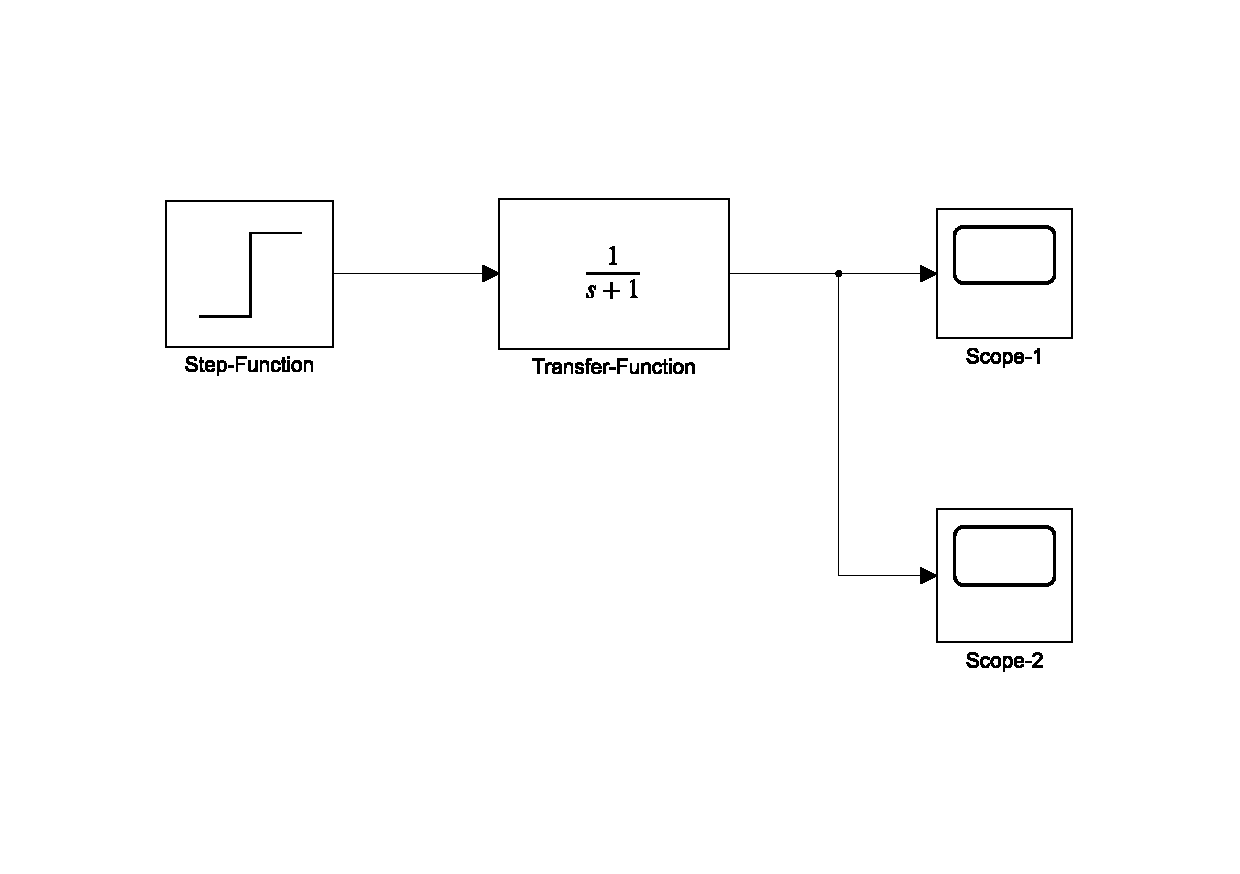
\includegraphics[width=8.5cm,valign=c]{MATLAB/Simulink/simulink_model.pdf}\hfill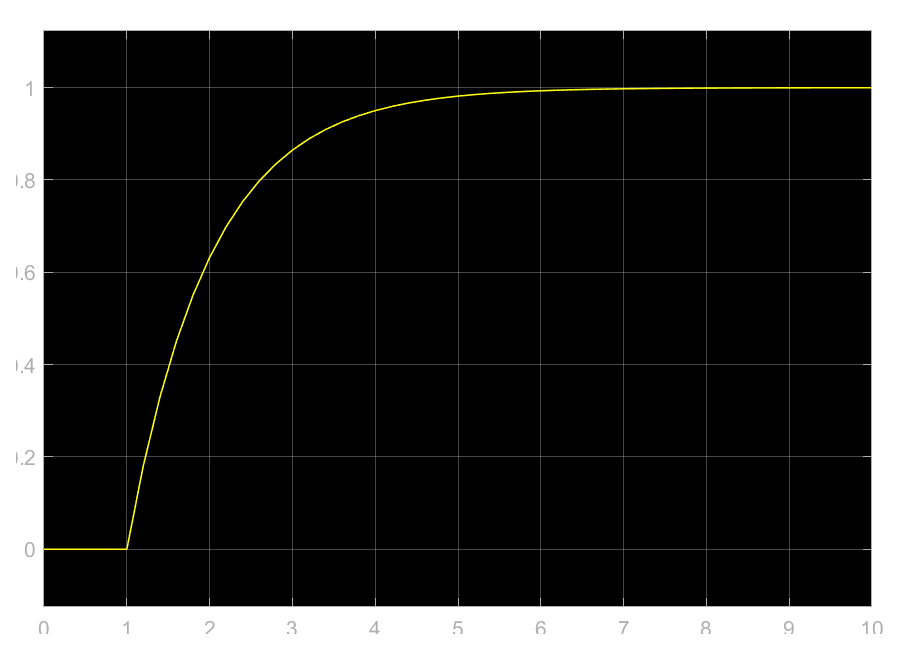
\includegraphics[width=8.5cm,valign=c]{MATLAB/Simulink/graph_example.eps}    
    \caption{Task One - System Model (left) and Graph Output (right)}
    \label{fig:example_model_graph}
\end{figure}

\pagebreak


\section{Arduino Code}
Arduino code is just as easily added, an example is displayed in Listing\ref{lis:arduino_example}. You will find the full code to this project \href{https://github.com/mjennings061/primary-engineer/tree/Wi-Fi}{here}!
\bigskip

{Arduino WiFi Based Code - NeoPixel File}
\lstinputlisting[style=Arduino, label={lis:arduino_example},caption={}]{Arduino/neopix.ino}


\newpage


\newpage
\setstretch{1}  % Reduce bibliography line spacing
\printbibliography
\end{document}
